
\section*{Introduction}

Terrestrial biodiversity is declining on a global scale\cite{leclere2020, ipbes2019, keck2025}, caused by land use change, natural resource exploitation, pollution, climate change, and invasive species \cite{keck2025,jaureguiberry2022}. Biodiversity loss threatens the stability of ecosystems and the services they provide, on which human prosperity depends\cite{cardinale2012}. The recently updated monitoring framework \cite{gbfmf2025} of the Global Biodiversity Framework \cite{gbf2022} (the GBF-MF) underscores the critical role of biodiversity indicators to halt and reverse this development \cite{affinito2024}. In parallel, companies are accelerating efforts to understand nature-related dependencies, impacts, and risks \cite{sbtn2020,tnfd2023,npi2025,goodsell2025}. Demand is therefore growing for robust, globally consistent indicators for assessing biodiversity change and its drivers \cite{burgess2024}.

While global biodiversity repositories contain increasing amounts of data, lingering geographic and taxonomic gaps make comprehensive biodiversity monitoring challenging \cite{hughes2021,chapman2024,boyd2023}. Statistical models that quantify how biodiversity correlates with environmental drivers and human pressures\cite{purvis2025} have the potential to fill data gaps through spatial projections. Models could thereby support national monitoring \cite{gbfmf2025}, global assessments \cite{ipbes2019}, and scenario analysis \cite{damania2023,leclere2020, zurell2025}, presenting a forward-looking complement to the GBF-MF headline indicators\cite{purvis2025,zurell2025}. However, modeling biodiversity dynamics at large scales raises questions about the generality of models: the extent to which inferences from a sample apply to the sampled ecological context at large, as well as to other contexts\cite{spake2022}. Generality is a major challenge when estimating effect sizes of drivers\cite{spake2022}, let alone when extending parameter inference to spatially explicit predictions of biodiversity. Ecological prediction is notably hard due to local dynamics emerging from a combination of evolutionary patterns, biotic and abiotic interactions, scale dependencies, and biological stochasticity \cite{maris2018}.

Challenges notwithstanding, scalable monitoring of biodiversity change and its drivers are key questions for biodiversity research\cite{purvis2025}. In this context, biodiversity is measured relative to some baseline condition in time or space, often using the concept of biodiversity intactness: ‘the average abundance of a large and diverse set of organisms in a given geographical area, relative to their reference populations’ \cite{scholes2005}. The intactness of a given location can be quantified using pressure-response models of species richness, abundance and composition, in relation to reference sites that are relatively ecologically intact. Global model-based intactness indicators, such as the Biodiversity Intactness Index (BII) \cite{newbold2015,newbold2016} and Mean Species Abundance (from GLOBIO) \cite{schipper2020}, have been widely adopted, for example by the GBF-MF \cite{gbfmf2025}, the Intergovernmental Science-Policy Platform on Biodiversity and Ecosystem Services (IPBES) \cite{ipbes2019}, and the private sector\cite{burgess2024}. This adoption underscores the value of biodiversity models to support policy and decision-making \cite{zurell2025,burgess2024,affinito2024,purvis2025}.

Efforts to develop large-scale, model-based indicators have advanced biodiversity modeling, generating important insights about the effects of human pressures\cite{newbold2015,schipper2020} with major value for conservation policy. Yet, there has also been critique against lack of agreement with other global metrics\cite{martin2019}, limited applicability in data-poor regions\cite{clements2025}, and insufficient model testing\cite{martin2019}. Considering their applied relevance, the use of pressure-response models for spatially explicit projections calls for more systematic evaluation of predictive performance. Evaluation is particularly important in this context, since data for global models relies on aggregation of many heterogeneous source studies into meta-databases. The spatial and taxonomic heterogeneity in study contexts, combined with gaps in underlying data, imply a need for extensive extrapolation to produce continuous output maps. Results from macroecological and species distribution modeling show that reasonable model performance can often be achieved when predicting in a context similar to the training data, while accuracy is typically much lower when predicting into new contexts \cite{roberts2017,meyer2021,meyer2022}. However, such results are generally based on much narrower contexts than the

\begin{figure}[H]
    \centering
    \noindent\rule{\linewidth}{0.4pt}\par\vspace{6pt}
    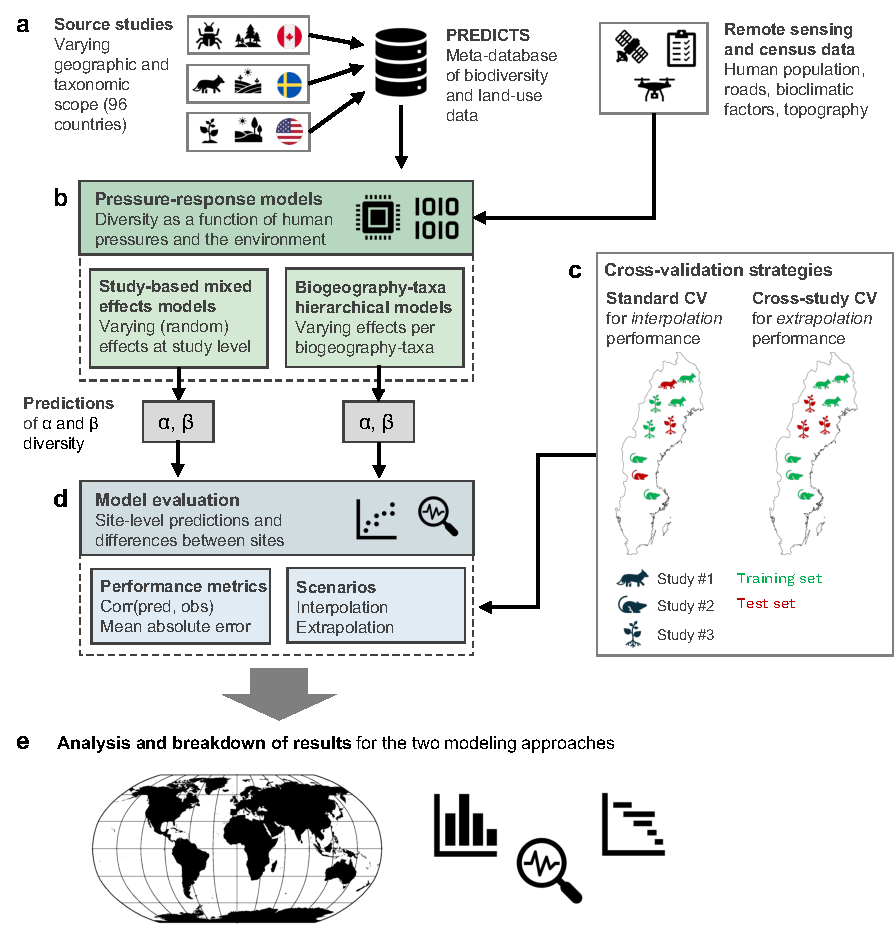
\includegraphics[width=0.96\linewidth]{figures/main/pipeline.pdf}
    \vspace{-10pt}
    \caption{\textbf{Data and model pipeline for this study.}
    \textbf{a}, Biodiversity and land-use data from 681 source studies comprising 25,987 sampling sites were joined with data on human population density, road network density, bioclimatic factors, and topography.
    \textbf{b}, We trained two statistical pressure-response models: 1) A generalized linear mixed effects model with human pressures as fixed effects, where study-level random effects accounted for other variation in the data. 2) A Bayesian hierarchical model with varying parameters at the biogeographic-taxonomic level, also including additional bioclimatic and topographic covariates. Geometric mean abundance was used to represent site-level alpha diversity, while beta diversity was calculated as the Bray-Curtis similarity between ecologically intact reference sites and other sites.
    \textbf{c}, Two cross-validation strategies were used: For interpolation (‘standard’ CV), folds were generated by splitting data at the site level, such that sites from a given study could be allocated to multiple folds. For extrapolation (cross-study validation), folds were based on splits at the study level, such that all sites from a given study only appeared in a single fold.
    \textbf{d}, Model accuracy was assessed through the correlation between predicted and observed values (Pearson’s $r$) and the mean absolute error (MAE).
    \textbf{e}, The results were analyzed to understand performance differences and issues across model types, scenarios and countries.
    \textit{Flag icons source: Freepik (CA, SE), iconset.co (US). Map source: The Transhumanist.}}
    \par\vspace{0pt}\noindent\rule{\linewidth}{0.4pt}
    \label{fig:pipeline}
\end{figure}

global extent and broad taxonomic scope evaluated here. The amplified data limitations that come with this\cite{hughes2021,chapman2024,boyd2023} makes evaluation more challenging\cite{depalma2021} but nonetheless important\cite{martin2019}. To our knowledge, this has not been done for pressure-based biodiversity models with a global scope.

Here we quantitatively evaluate the generality of two different pressure-response models for projecting site-level biodiversity (overview in \autoref{fig:pipeline}). Generality is operationalized as model accuracy when making spatially explicit, out-of-sample predictions in sampled ecological contexts (generalizability) as well as in other contexts (transferability). We leverage species inventory data from 25,987 sites in 96 countries, with broad taxonomic coverage. The data originates from 681 studies collated in the widely used PREDICTS database\cite{hudson2017} (see \autoref{fig:predicts_data}). The first model uses a mixed effects structure\cite{harrison2018} with human pressures as fixed effects, estimated on average across all sites, and random effects to account for variation between studies. Such model structures are common in biodiversity meta-analysis\cite{spake2022} and used in different indicators \cite{newbold2015,schipper2020}. In the second model, we group data by biogeographic and taxonomic attributes in a hierarchical structure. Model parameters are estimated individually for each group, while sharing information across. Environmental variables complement the human pressures to create a richer model. The rationale is to learn from more contextual information that can be used for out-of-sample prediction. Our aim is to explore the implications of biodiversity data availability and model design on generality, providing insights for future work on large-scale biodiversity models.
